%%%%%%%%%%%%%%%%%%%%%%%%%%%%%%%%%%%%%%%%%%%%%%%%%%%%%%%%%%%
%\documentclass[xcolor=x11names,compress]{beamer}
\documentclass[xcolor=x11names,  aspectratio=169, compress]{beamer}
%% General document
\usepackage{graphicx, subfig}
%% Beamer Layout
\useoutertheme[subsection=false,shadow]{miniframes}
\useinnertheme{default}
\usefonttheme{serif}
\usepackage{palatino}

%%%%%%% Mes Packages %%%%%%%%%%%%%%%%
%\usepackage[french]{babel}
\usepackage[T1]{fontenc}
\usepackage{color}
\usepackage{xcolor}

\usepackage{dsfont} % Pour indicatrice
\usepackage{url}
\usepackage{multirow}
\usepackage[normalem]{ulem}   % For strike out text
%%%% TiKz
\usepackage{tikz}
\usetikzlibrary{positioning}

% Natbib for clean bibliography
\usepackage[comma,authoryear]{natbib}

%remove the icon
\setbeamertemplate{bibliography item}{}

%remove line breaks
\setbeamertemplate{bibliography entry title}{}
\setbeamertemplate{bibliography entry location}{}
\setbeamertemplate{bibliography entry note}{}

%% ------ MEs couleurs --------
\definecolor{vert}{rgb}{0.1,0.7,0.2}
\definecolor{brique}{rgb}{0.7,0.16,0.16}
\definecolor{gris}{rgb}{0.7, 0.75, 0.71}
\definecolor{twitterblue}{rgb}{0, 0.42, 0.58}
\definecolor{airforceblue}{rgb}{0.36, 0.54, 0.66}
\definecolor{siap}{RGB}{3,133, 200}


%%%%%%%%%%%%%%%%% BEAMER PACKAGE %%%%%%%

\setbeamercolor{itemize item}{fg=siap}
%\setbeamercolor{itemize subitem}{fg=blue}
%\setbeamercolor{itemize subsubitem}{fg=cyan}

\setbeamerfont{title like}{shape=\scshape}
\setbeamerfont{frametitle}{shape=\scshape}

\setbeamercolor*{lower separation line head}{bg=DeepSkyBlue4}
\setbeamercolor*{normal text}{fg=black,bg=white}
\setbeamercolor*{alerted text}{fg=siap}
\setbeamercolor*{example text}{fg=black}
\setbeamercolor*{structure}{fg=black}
\setbeamercolor*{palette tertiary}{fg=black,bg=black!10}
\setbeamercolor*{palette quaternary}{fg=black,bg=black!10}

% Set the header color to SIAP's color
\setbeamercolor*{frametitle}{fg=siap}

%remove navigation symbols
\setbeamertemplate{navigation symbols}{}

\renewcommand{\(}{\begin{columns}}
\renewcommand{\)}{\end{columns}}
\newcommand{\<}[1]{\begin{column}{#1}}
\renewcommand{\>}{\end{column}}

%% Add footer with logo
\setbeamertemplate{footline}{%
  \begin{beamercolorbox}[wd=\paperwidth,ht=2.5ex,dp=1.125ex,%
    leftskip=.3cm,rightskip=.3cm plus1fil]{author in head/foot}
    
\includegraphics[height=5ex]{SIAP_logo_Big.png}\hfill
    \insertshortauthor\hfill\insertshorttitle\hfill  \textcolor{siap}{\textit{\insertframenumber}}
  \end{beamercolorbox}%
}


% Path for the graphs
\graphicspath{
{Graphics/}
{../../../../Visualisation/Presentations/Graphics/Logos}
{../../Visualisation/Presentations/Graphics/}
{c:/Gitmain/MLCourse/UNML/Module0/M0_files/figure-html/}
{c:/Chris/UN-ESCAP/MyCourses2022/MLOS2022/Slides/Graphics/}
{c:/Chris/UN-ESCAP/MyCourses2023/BigDataKostat/Slides/Graphics/}
{../../../../Visualisation/Presentations/Graphics/SIAP/icons/}
{c:/Chris/UN-ESCAP/SIAP-E-learning/Resources/Pictos/}
 }

\title{\textcolor{siap}{Big Data and Data Science for Gender Statistics\\ in Asia and the Pacific\\ \vspace{0.5cm} }}

\subtitle{\textcolor{brique}{\Large{From Text to Data}}}
\author{Christophe Bontemps}
\institute{ 
\includegraphics[height=10ex]{SIAP_logo_Big.png}}
\date{}

\begin{document}

% Slide 1: Title Slide
\begin{frame}
    \titlepage
\end{frame}

%-----------------------------------------
\begin{frame}{Motivation}
\begin{itemize}
    \item Text is everywhere — reports, media, policy, and statistics.
    \item We increasingly need to extract \textbf{structured data} from text.
    \item LLMs (like BERT,RoBERTa, GPT) make this possible.
\end{itemize}

\begin{center}
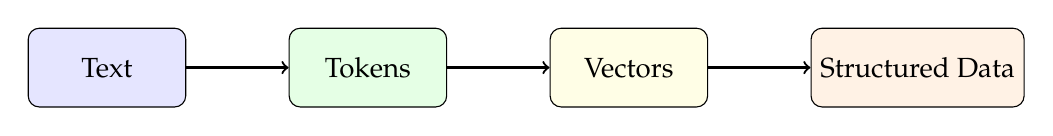
\begin{tikzpicture}[node distance=1.3cm, every node/.style={rounded corners, draw, align=center, minimum width=2cm, minimum height=1cm}]
\node[fill=blue!10] (text) {Text};
\node[fill=green!10, right=of text] (tokens) {Tokens};
\node[fill=yellow!10, right=of tokens] (vectors) {Vectors};
\node[fill=orange!10, right=of vectors] (data) {Structured Data};
\draw[->, thick] (text) -- (tokens);
\draw[->, thick] (tokens) -- (vectors);
\draw[->, thick] (vectors) -- (data);
\end{tikzpicture}
\end{center}
\end{frame}

%-----------------------------------------
\begin{frame}{Example Text: Gender and Statistics}
\begin{block}{Example:}
\emph{"In 2023, 45\% of women in the region reported experiencing violence. 
The Ministry launched a program to address femicide and improve data collection on gender-based violence."}
\end{block}

\begin{center}
\begin{tabular}{l l}
\toprule
\textbf{Concept} & \textbf{Extracted Value} \\
\midrule
Year & 2023 \\
Population & Women \\
Topic & Gender-based violence \\
Specific concept & Femicide \\
\bottomrule
\end{tabular}
\end{center}
\end{frame}

%-----------------------------------------
\begin{frame}{Step 1: Tokenization}
\begin{itemize}
  \item Split text into small units — tokens.
  \item Tokens can be words or subwords.
\end{itemize}
\begin{block}{Example}
\texttt{"The Ministry launched a program"} \\ $\rightarrow$  
[\texttt{The}], [\texttt{Ministry}], [\texttt{launched}], [\texttt{a}], [\texttt{program}]
\end{block}

\begin{center}
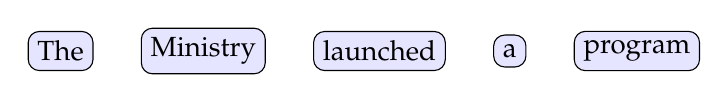
\begin{tikzpicture}[node distance=0.6cm]
\node[draw, rounded corners, fill=blue!10] (t1) {The};
\node[draw, rounded corners, fill=blue!10, right=of t1] (t2) {Ministry};
\node[draw, rounded corners, fill=blue!10, right=of t2] (t3) {launched};
\node[draw, rounded corners, fill=blue!10, right=of t3] (t4) {a};
\node[draw, rounded corners, fill=blue!10, right=of t4] (t5) {program};
\end{tikzpicture}
\end{center}
\end{frame}

%-----------------------------------------
\begin{frame}{Step 2: Lemmatization}
\begin{itemize}
  \item Reduces words to their base form (lemma).
  \item Groups variations of the same concept.
\end{itemize}

\begin{block}{Example}
\texttt{"women"} → \texttt{"woman"} \quad 
\texttt{"reporting"} → \texttt{"report"}
\end{block}

\begin{center}
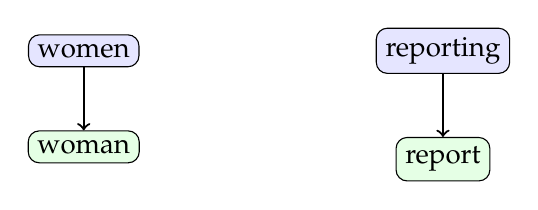
\begin{tikzpicture}
\node[draw, fill=blue!10, rounded corners] (a) {women};
\node[draw, fill=green!10, below=0.8cm of a, rounded corners] (b) {woman};
\draw[->, thick] (a) -- (b);

\node[draw, fill=blue!10, rounded corners, right=3cm of a] (c) {reporting};
\node[draw, fill=green!10, below=0.8cm of c, rounded corners] (d) {report};
\draw[->, thick] (c) -- (d);
\end{tikzpicture}
\end{center}
\end{frame}


%-----------------------------------------
\begin{frame}{Step 3a: Vectorization}
\begin{itemize}
    \item Computers cannot "understand" raw text.
    \item[$\hookrightarrow$] We need numeric representations to apply mathematical operations.
    \item Each token $\rightarrow$ \textbf{vector}  (numbers).
\end{itemize}

\begin{center}
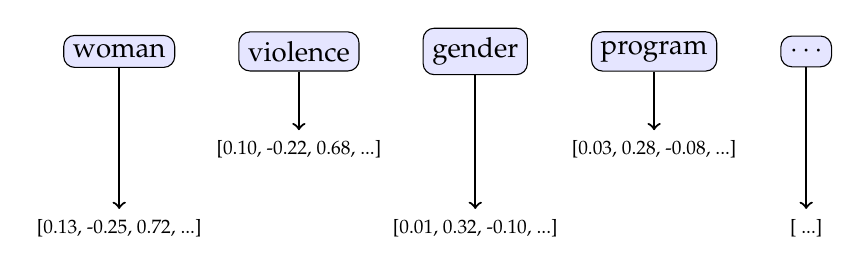
\begin{tikzpicture}[node distance=0.8cm]
\node[draw, fill=blue!10, rounded corners] (t1) {woman};
\node[draw, fill=blue!10, rounded corners, right=of t1] (t2) {violence};
\node[draw, fill=blue!10, rounded corners, right=of t2] (t3) {gender};
\node[draw, fill=blue!10, rounded corners, right=of t3] (t4) {program};
\node[draw, fill=blue!10, rounded corners, right=of t4] (t5) {$\cdots$};

\draw[->, thick] (t1) -- ++(0,-2.0) node[below] {\scriptsize [0.13, -0.25, 0.72, ...]};
\draw[->, thick] (t2) -- ++(0,-1.0) node[below] {\scriptsize [0.10, -0.22, 0.68, ...]};
\draw[->, thick] (t3) -- ++(0,-2.0) node[below] {\scriptsize [0.01, 0.32, -0.10, ...]};
\draw[->, thick] (t4) -- ++(0,-1.0) node[below] {\scriptsize [0.03, 0.28, -0.08, ...]};
\draw[->, thick] (t5) -- ++(0,-2.0) node[below] {\scriptsize [ ...]};

\end{tikzpicture}
\end{center}
\end{frame}

\begin{frame}{Step 3b: From Words to Numbers}
\begin{itemize}
   \item Each token $w_i$ is represented as a vector in $\mathbb{R}^{d}$:
    \[
        w_i \mapsto \vec{v_i} = [v_{i1}, v_{i2}, \dots, v_{id}]
    \]
    \item[] \hfill {\scriptsize  \textit{Typically $d$ = 768 in RoBERTa} }
    \item[$\hookrightarrow$] Example: \text{"woman"} = [0.13, -0.25, 0.72, \ldots]
\end{itemize}


\centering
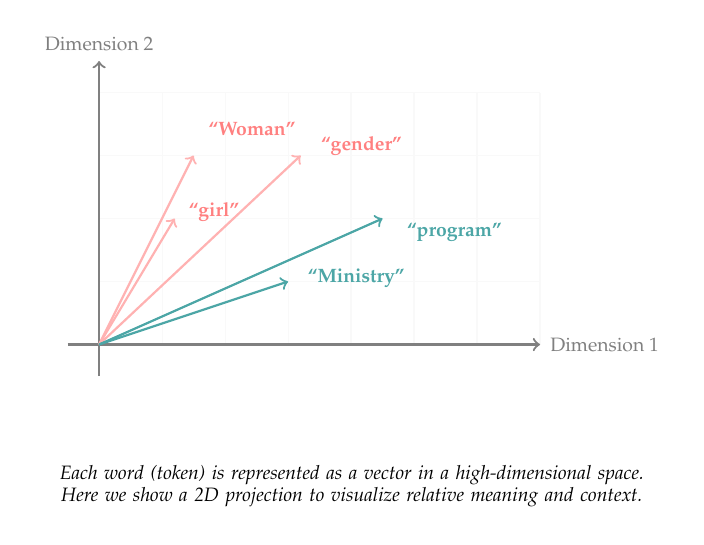
\begin{tikzpicture}[scale=0.8, every node/.style={font=\scriptsize}]
   % Grid for context (always before drawing  layers!!) 
   \draw[gray!5, step=1] (0,0) grid (7,4);
    % Axes
    \draw[->, thick,  black!50] (-0.5,0) -- (7,0) node[right, black!50 ]{Dimension 1};
    \draw[->, thick,  black!50] (0,-0.5) -- (0,4.5) node[above, black!50]{Dimension 2};
    % Tokens represented as vectors
    \draw[->, thick, red!30] (0,0) -- (1.5,3) node[pos=1.05, above right, red!50]{\textbf{“Woman”}};
    \draw[->, thick, red!30] (0,0) -- (1.2,2) node[pos=1.05, right, red!50]{\textbf{“girl”}};
    \draw[->, thick, red!30] (0,0) -- (3.2,3) node[pos=1.05, right, red!50]{\textbf{“gender”}};
    \draw[->, thick, teal!70] (0,0) -- (4.5,2) node[pos=1.05, below right, teal!70]{\textbf{“program”}};
     \draw[->, thick, teal!70] (0,0) -- (3,1) node[pos=1.05, right,teal!70]{\textbf{“Ministry”}};

    % Caption
    \node[align=center, below=1cm of current bounding box.south, text width=8cm]
        {\textit{Each word (token) is represented as a vector in a high-dimensional space. \\ 
        Here we show a 2D projection to visualize relative meaning and context.}};
\end{tikzpicture}
\end{frame}

%-----------------------------------------
\begin{frame}{Step 3c: Vector Space ``Embeds'' Meaning}
\begin{itemize}
    \item Tokens with similar meaning are close in vector space.
    \[
        \text{similar}(w_i, w_j) \approx \text{cos\_sim}(\vec{v_i}, \vec{v_j})
    \]
\end{itemize}

\begin{center}
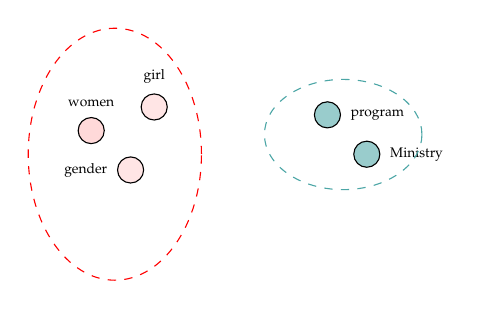
\begin{tikzpicture}[scale=1.0]
% Femicide cluster
\node[circle, draw, fill=red!15, label=above:{\tiny women}] (a) at (0,0) {};
\node[circle, draw, fill=red!10, label=above:{\tiny girl}] (b) at (0.8,0.3) {};
\node[circle, draw, fill=red!10, label=left:{\tiny gender}] (c) at (0.5,-0.5) {};

% Animal cluster
\node[circle, draw, fill=teal!40, label=right:{\tiny program}] (d) at (3,0.2) {};
\node[circle, draw, fill=teal!40, label=right:{\tiny Ministry}] (e) at (3.5,-0.3) {};

\draw[dashed, red] (0.3,-0.3) ellipse (1.1cm and 1.6cm);
\draw[dashed, teal!70] (3.2,-0.05) ellipse (1.0cm and 0.7cm);
\end{tikzpicture}
\end{center}
 \hfill {\scriptsize  \textit{ Cosine similarity is often used to measure similarity:
$
\text{cos\_sim}(\vec{v_1}, \vec{v_2}) = \frac{\vec{v_1} \cdot \vec{v_2}}{||\vec{v_1}|| \, ||\vec{v_2}||} 
$  }}
\end{frame}

%-----------------------------------------


%-----------------------------------------
\begin{frame}{Step 3d: Embedding Tokens from Example Text}

\emph{"In 2023, 45\% of women in the region reported experiencing violence. 
The Ministry launched a program to address femicide and improve data collection on gender-based violence."} \\
\vspace{0.5cm}

\begin{itemize}
    \item Tokenized: \texttt{[ "women", "program", "violence", $\cdots$]}
    \item Vectorized: Each token $\rightarrow$ $\vec{v} \in \mathbb{R}^{768}$ 
    \item Semantic proximity: \\
    \texttt{"women"} and \texttt{"gender"} are closer than\\ \texttt{"women"} and \texttt{"program"}
\end{itemize}

\begin{center}
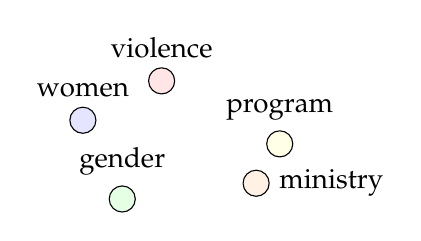
\begin{tikzpicture}[scale=1.0]
\node[circle, draw, fill=blue!10, label=above:{women}] (a) at (0,0) {};
\node[circle, draw, fill=red!10, label=above:{violence}] (b) at (1,0.5) {};
\node[circle, draw, fill=yellow!10, label=above:{program}] (c) at (2.5,-0.3) {};
\node[circle, draw, fill=green!10, label=above:{gender}] (d) at (0.5,-1) {};
\node[circle, draw, fill=orange!10, label=right:{ministry}] (e) at (2.2,-0.8) {};
\end{tikzpicture}
\end{center}

\end{frame}


%-----------------------------------------
\begin{frame}{Step 4: Contextual Embeddings with RoBERTa}
\begin{itemize}
  \item RoBERTa creates \textbf{context-aware} representations.
  \item Same word can mean different things depending on its context.
  \item Context will be included in the representation of each word-token
\end{itemize}

\begin{block}{Example}
\texttt{"She reports on femicide"}  
\texttt{"He reports on pesticide use"}
\end{block}

\begin{center}
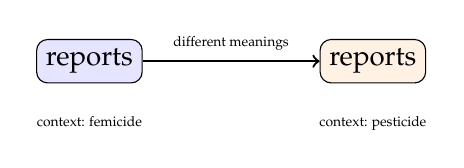
\begin{tikzpicture}[scale=1.2]
% Sentence 1
\node[draw, fill=blue!10, rounded corners] (r1) at (0,0) {reports};
\node[below=0.3cm of r1] {\tiny context: femicide};

% Sentence 2
\node[draw, fill=orange!10, rounded corners] (r2) at (3,0) {reports};
\node[below=0.3cm of r2] {\tiny context: pesticide};

\draw[->, thick] (r1) -- (r2) node[midway, above] {\tiny different meanings};
\end{tikzpicture}
\end{center}
\end{frame}

%-----------------------------------------


%-----------------------------------------
\begin{frame}{Pipeline Summary}
\begin{center}
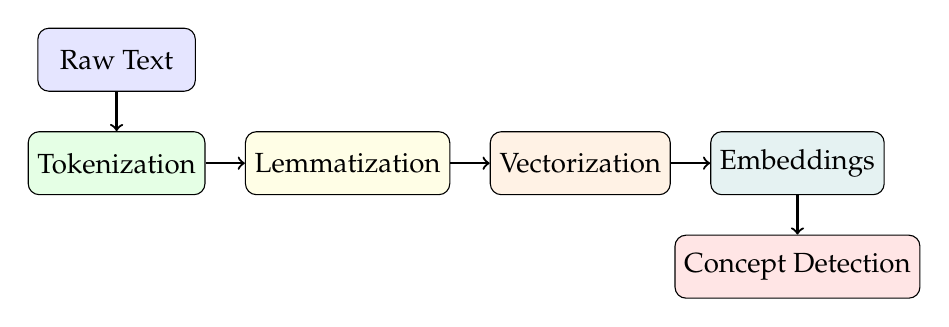
\begin{tikzpicture}[node distance=0.5cm, every node/.style={draw, rounded corners, minimum width=2cm, minimum height=0.8cm, align=center}]
\node[fill=blue!10] (a) {Raw Text};
\node[fill=green!10, below=of a] (b) {Tokenization};
\node[fill=yellow!10, right=of b] (c) {Lemmatization};
\node[fill=orange!10, right=of c] (d) {Vectorization};
\node[fill=teal!10, right=of d] (e) {Embeddings};
\node[fill=red!10, below=of e] (f) {Concept Detection};
\draw[->, thick] (a) -- (b);
\draw[->, thick] (b) -- (c);
\draw[->, thick] (c) -- (d);
\draw[->, thick] (d) -- (e);
\draw[->, thick] (e) -- (f);
\end{tikzpicture}
\end{center}
\end{frame}

%-----------------------------------------
\begin{frame}{Conclusion}
\begin{itemize}
  \item LLMs map words into high-dimensional space.
  \item They rely on tokenization, lemmatization, and vectorization.
  \item Context-aware models like RoBERTa detect meaning dynamically.
\end{itemize}

\begin{center}
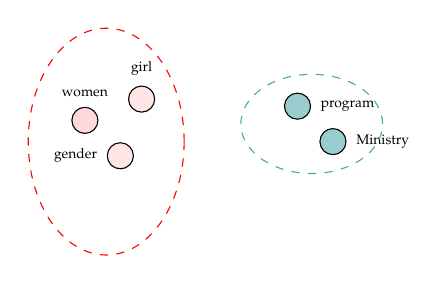
\begin{tikzpicture}[scale=0.9]
% Femicide cluster
\node[circle, draw, fill=red!15, label=above:{\tiny women}] (a) at (0,0) {};
\node[circle, draw, fill=red!10, label=above:{\tiny girl}] (b) at (0.8,0.3) {};
\node[circle, draw, fill=red!10, label=left:{\tiny gender}] (c) at (0.5,-0.5) {};

% Animal cluster
\node[circle, draw, fill=teal!40, label=right:{\tiny program}] (d) at (3,0.2) {};
\node[circle, draw, fill=teal!40, label=right:{\tiny Ministry}] (e) at (3.5,-0.3) {};

\draw[dashed, red] (0.3,-0.3) ellipse (1.1cm and 1.6cm);
\draw[dashed, teal!70] (3.2,-0.05) ellipse (1.0cm and 0.7cm);
\end{tikzpicture}
\end{center}
\begin{itemize}
  \item Terms like \textbf{women}, \textbf{girl}, and \textbf{gender} cluster together 
reflecting semantic proximity in the model’s representation.
\end{itemize}
\end{frame}

\begin{frame}{Example}
\begin{itemize}
    \item[] Sentence 1:  \texttt{“A woman was stabbed by her husband”}
    \item[] Sentence 2:   \texttt{“He stabbed the steak with a knife”}
    \item The original word (token) \texttt{"stabbed"} is apparently the same token
    \item It gets a different vector in the 768d-space in each sentence, bearing (\textit{embedding}) context.
\end{itemize}
 \centering
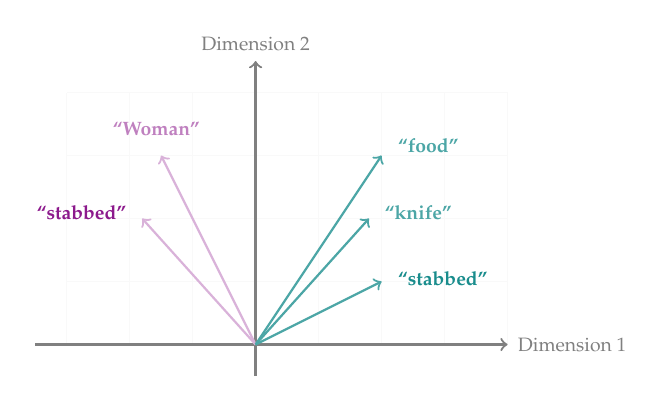
\begin{tikzpicture}[scale=0.8, every node/.style={font=\scriptsize}]
   % Grid for context (always first!)
   \draw[gray!5, step=1] (0,0) grid (7,4);
    % Axes
    \draw[->, thick,  black!50] (-0.5,0) -- (7,0) node[right, black!50 ]{Dimension 1};
    \draw[->, thick,  black!50] (3,-0.5) -- (3,4.5) node[above, black!50]{Dimension 2};
    
    % Tokens represented as vectors
    \draw[->, thick, violet!30] (3,0) -- (1.5,3) node[pos=1.05, above, violet!50]{\textbf{“Woman”}};
    \draw[->, thick, violet!30] (3,0) -- (1.2,2) node[pos=1.05, left, violet!90]{\textbf{“stabbed”}};
    \draw[->, thick, teal!70] (3,0) -- (5,3) node[pos=1.05, right, teal!70]{\textbf{“food”}};
    \draw[->, thick, teal!70] (3,0) -- (4.8,2) node[pos=1.05, right, teal!70]{\textbf{“knife”}};
     \draw[->, thick, teal!70] (3,0) -- (5,1) node[pos=1.05, right,teal!90]{\textbf{“stabbed”}};
\end{tikzpicture}
\end{frame}

%%%%%%%%%%%%%%%%%%%%%%%%
\begin{frame}{Details on Step 2: How Are Token Embeddings Computed?}
% See https://www.3blue1brown.com/lessons/gpt#what-is-a-gpt-model
  Each token (e.g., \texttt{femicide}, \texttt{violence}) is represented in a very large space (\textit{dim = 768}) and integrate other contextual elements:
  \[
  \text{InputEmbedding}(x_i) =
  E_{\text{token}}(x_i) + E_{\text{position}}(i) + E_{\text{segment}}(i)
  \]
  These\textit{\textbf{"embeddings"}} are passed through a stack of Transformer layers \textit{(deep-learning}) to determine their best position in the vector space.
  
  \vspace{0.4cm}
  \begin{block}{\textbf{Goal}}
  Capture contextual meaning: “femicide” should be near “women” and \textit{unrelated} to “program”.
  \end{block}
\end{frame}

\begin{frame}{Machine Learning Perspective}
\small
  \[
  f_\theta: \text{Token} \rightarrow \mathbb{R}^{768}
  \]
  \vspace{0.2cm}
  where $f_\theta$ is trained to minimize the loss:
  \[
  \min_\theta \sum_{(x,y)} -\log P_\theta(y | x_{\text{masked}})
  \]
 With ML (deep learning):
  \begin{itemize}
    \item The model learns to predict missing words (e.g., “femicide”) from context. %Through this process, it learns semantic relationships (similar words get similar vectors) through millions of examples.\\
     \item Each 768-dimensional vector, $\theta$, is the output of a trained function, capturing how the model represents token’s meaning in context.
      \item Including semantic similarity (e.g., “woman”, “girl”)
      \item Including contextual meaning (“food” vs “crime” context)
  \end{itemize}
 \hfill {\tiny Why 768? It’s the \textbf{hidden size} of the RoBERTa model\\
\hfill large enough to encode meaning, small enough for efficiency.}
\end{frame}


\begin{frame}{ML Pretraining:  Predicting Missing Tokens}
\centering
\textbf{Goal:} Learn context and meaning by predicting masked words (like imputation). \\[0.4cm]

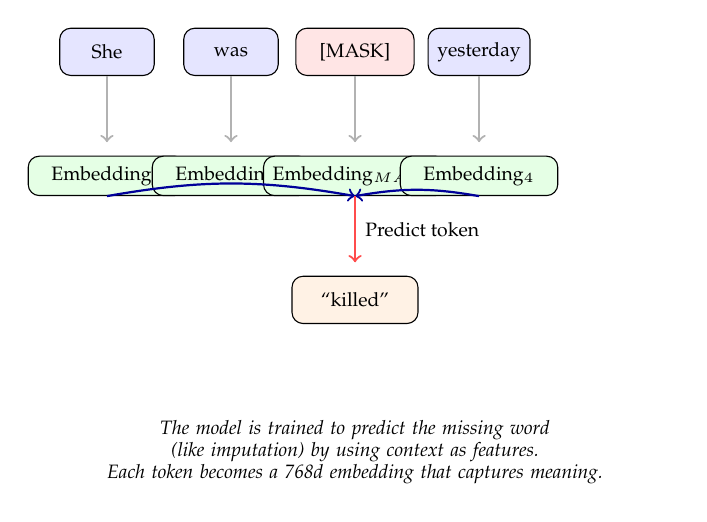
\begin{tikzpicture}[scale=1.05, every node/.style={font=\scriptsize}]
    % Sentence
    \node[draw, rounded corners, fill=blue!10, minimum width=1.2cm, minimum height=0.6cm] (t1) at (0,0) {She};
    \node[draw, rounded corners, fill=blue!10, minimum width=1.2cm, minimum height=0.6cm] (t2) at (1.5,0) {was};
    \node[draw, rounded corners, fill=red!10, minimum width=1.5cm, minimum height=0.6cm] (mask) at (3,0) {[MASK]};
    \node[draw, rounded corners, fill=blue!10, minimum width=1.2cm, minimum height=0.6cm] (t4) at (4.5,0) {yesterday};

    % Arrows to embedding space
    \foreach \i in {t1,t2,mask,t4}{
        \draw[->, thick, gray!60] (\i.south) -- ++(0,-0.8);
    }

    % Embeddings (vectors)
    \node[draw, fill=green!10, rounded corners, minimum width=2cm, minimum height=0.5cm] (e1) at (0,-1.5) {Embedding$_1$};
    \node[draw, fill=green!10, rounded corners, minimum width=2cm, minimum height=0.5cm] (e2) at (1.5,-1.5) {Embedding$_2$};
    \node[draw, fill=green!10, rounded corners, minimum width=2cm, minimum height=0.5cm] (em) at (3,-1.5) {Embedding$_{MASK}$};
    \node[draw, fill=green!10, rounded corners, minimum width=2cm, minimum height=0.5cm] (e4) at (4.5,-1.5) {Embedding$_4$};

    % Context attention arrows (simplified)
    \draw[->, thick, blue!60!black, bend left=15] (e1.south) to[bend left=10] (em.south);
    \draw[->, thick, blue!60!black, bend right=15] (e4.south) to[bend right=10] (em.south);

    % Output prediction
    \draw[->, thick, red!70] (em.south) -- ++(0,-0.8) node[midway,right,black]{\scriptsize Predict token};
    \node[draw, fill=orange!10, rounded corners, minimum width=1.6cm, minimum height=0.6cm] (out) at (3,-3) {“killed”};

    % Caption
    \node[align=center, below=1.1cm of out, text width=8cm]{
        \textit{The model is trained  to predict the missing word (like imputation) by using context as features.\\
        Each token becomes a 768d embedding that captures meaning.}
    };
\end{tikzpicture}
\end{frame}



\begin{frame}{ML Fine-tuning – From Tokens to Prediction}
\centering
\textbf{Goal:} Use vector representations to classify whether a text mentions \textit{femicide}. \\[0.4cm]

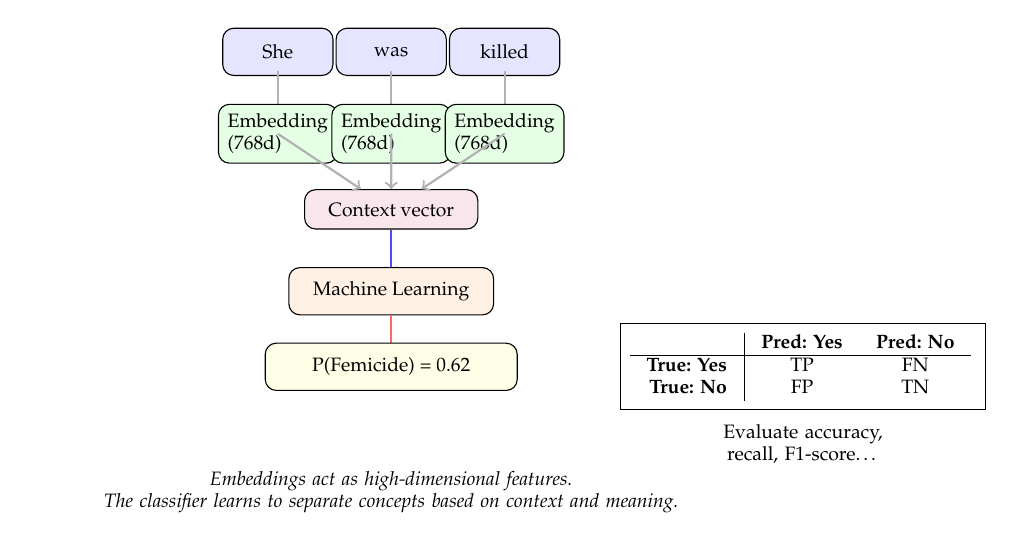
\begin{tikzpicture}[scale=0.8, every node/.style={font=\scriptsize}]
    % Input sentence
    \node[draw, rounded corners, fill=blue!10, minimum width=1.4cm, minimum height=0.6cm] (t1) at (0,0) {She};
    \node[draw, rounded corners, fill=blue!10, minimum width=1.4cm, minimum height=0.6cm] (t2) at (1.8,0) {was};
    \node[draw, rounded corners, fill=blue!10, minimum width=1.4cm, minimum height=0.6cm] (t3) at (3.6,0) {killed};

    % Arrows to embeddings
    \foreach \x in {0,1.8,3.6}{
        \draw[->, thick, gray!60] (\x,-0.3) -- (\x,-1);
        \node[draw, fill=green!10, rounded corners, align=left] at (\x,-1.3) {  Embedding \\ (768d) };
    }

    % Aggregation / context vector
    \node[draw, fill=purple!10, rounded corners, minimum width=2.2cm, minimum height=0.5cm] (agg) at (1.8,-2.5) {Context vector};
    \draw[->, thick, gray!60] (0,-1.3) -- (agg);
    \draw[->, thick, gray!60] (1.8,-1.3) -- (agg);
    \draw[->, thick, gray!60] (3.6,-1.3) -- (agg);

    % Classifier
    \draw[->, thick, blue!70] (agg.south) -- ++(0,-0.7);
    \node[draw, fill=orange!10, rounded corners, minimum width=2.6cm, minimum height=0.6cm] (cls) at (1.8,-3.8) {Machine Learning};

    % Output probabilities
    \draw[->, thick, red!60] (cls.south) -- ++(0,-0.7);
    \node[draw, fill=yellow!10, rounded corners, minimum width=3.2cm, minimum height=0.6cm] (out) at (1.8,-5) {P(Femicide) = 0.62};

    % Confusion matrix (to the right)
    \node[draw, fill=white, below right=0.1cm and 1.6cm of cls, align=center] (cm) {
        \begin{tabular}{r|cc}
         & \textbf{Pred: Yes} & \textbf{Pred: No} \\
        \hline
        \textbf{True: Yes} & TP & FN \\
        \textbf{True: No} & FP & TN \\
        \end{tabular}
    };
    \node[below=0.05cm of cm, text width=3.3cm, align=center] {
        \scriptsize Evaluate accuracy, recall, F1-score…
    };

    % Caption
    \node[align=center, below=0.9cm of out, text width=9cm]{
        \textit{Embeddings act as high-dimensional features.\\
        The classifier learns to separate concepts based on context and meaning.}
    };
\end{tikzpicture}
\end{frame}



\begin{frame}{Embedings space is meaningful }
\begin{itemize}
    \item After training, Directions in this space have meaning.
    \item The difference between vectors can help  finding other words: 
     $$ E(Queen) - E(King) \simeq E(Woman) - E(Man) $$
   
\end{itemize}
 \centering
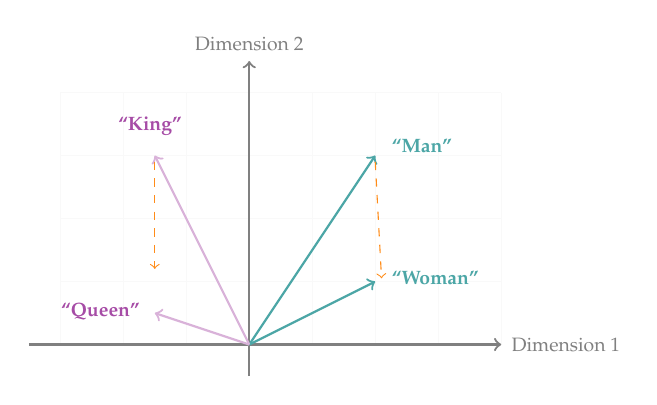
\begin{tikzpicture}[scale=0.8, every node/.style={font=\scriptsize}]
   % Grid for context (always first!)
   \draw[gray!5, step=1] (0,0) grid (7,4);
    % Axes
    \draw[->, thick,  black!50] (-0.5,0) -- (7,0) node[right, black!50 ]{Dimension 1};
    \draw[->, thick,  black!50] (3,-0.5) -- (3,4.5) node[above, black!50]{Dimension 2};
    
    % Tokens represented as vectors
   
    \draw[->, thick, teal!70] (3,0) -- (5,3) node[pos=1.05, right, teal!70]{\textbf{“Man”}};
    \draw[->, thick, teal!70] (3,0) -- (5,1) node[pos=1.05, right,teal!70]{\textbf{“Woman”}};
    \draw[->, thick, violet!30] (3,0) -- (1.5,3) node[pos=1.05, above, violet!70]{\textbf{“King”}};
    \draw[->, thick, violet!30] (3,0) -- (1.5,0.5) node[pos=1.05, left, violet!70]{\textbf{“Queen”}};
    \draw[->, dashed, orange!90] (5,2.9) -- (5.1,1.05) node[pos=1.05, right, teal!70]{};
    \draw[->, dashed, orange!90] (1.5,2.9) -- (1.5, 1.2) node[pos=1.05, right, teal!70]{};
    % \draw[->, thick, violet!30] (3,0) -- (1.5,3) node[pos=1.05, above, violet!50]{\textbf{“Woman”}};
\end{tikzpicture}
\end{frame}

\begin{frame}{Embeddings space is meaningful }
\begin{itemize}
    \item The difference between vectors can help  finding other words: 
     $$ E(Femicide) \simeq E(Murder) + E(Woman) - E(Man) $$
   
\end{itemize}
 \centering
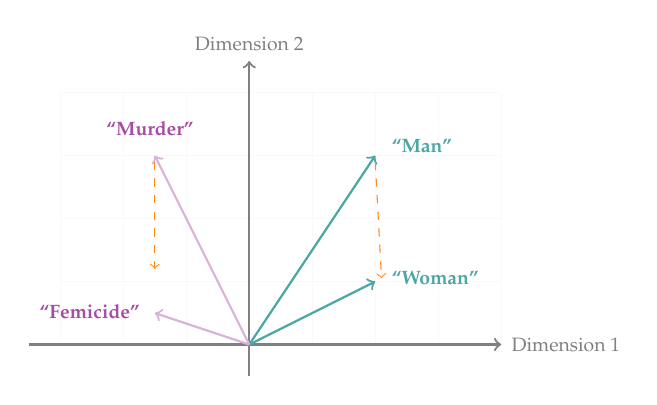
\begin{tikzpicture}[scale=0.8, every node/.style={font=\scriptsize}]
   % Grid for context (always first!)
   \draw[gray!5, step=1] (0,0) grid (7,4);
    % Axes
    \draw[->, thick,  black!50] (-0.5,0) -- (7,0) node[right, black!50 ]{Dimension 1};
    \draw[->, thick,  black!50] (3,-0.5) -- (3,4.5) node[above, black!50]{Dimension 2};
    
    % Tokens represented as vectors
   
    \draw[->, thick, teal!70] (3,0) -- (5,3) node[pos=1.05, right, teal!70]{\textbf{“Man”}};
    \draw[->, thick, teal!70] (3,0) -- (5,1) node[pos=1.05, right,teal!70]{\textbf{“Woman”}};
    \draw[->, thick, violet!30] (3,0) -- (1.5,3) node[pos=1.05, above, violet!70]{\textbf{“Murder”}};
    \draw[->, thick, violet!30] (3,0) -- (1.5,0.5) node[pos=1.05, left, violet!70]{\textbf{“Femicide”}};
    \draw[->, dashed, orange!90] (5,2.9) -- (5.1,1.05) node[pos=1.05, right, teal!70]{};
    \draw[->, dashed, orange!90] (1.5,2.9) -- (1.5, 1.2) node[pos=1.05, right, teal!70]{};
    % \draw[->, thick, violet!30] (3,0) -- (1.5,3) node[pos=1.05, above, violet!50]{\textbf{“Woman”}};
\end{tikzpicture}\\

\hfill \textcolor{gris}{ \scriptsize See \href{https://www.3blue1brown.com/lessons/gpt#title}{\textbf{3Blue1Brown.com}}  for more details}
\end{frame}



\end{document}
